\documentclass{article}

\usepackage[hyphens]{url}
\usepackage[hidelinks]{hyperref}

\usepackage[utf8]{inputenc}
\usepackage[T1]{fontenc}
\usepackage[british]{babel}
\usepackage{booktabs}

\usepackage[all]{foreign}
\renewcommand{\foreignfullfont}{}
\renewcommand{\foreignabbrfont}{}

\usepackage{newclude}
\usepackage{import}

\usepackage[strict]{csquotes}
\usepackage[single]{acro}

\usepackage[natbib,style=alphabetic,maxbibnames=99]{biblatex}
\addbibresource{slides.bib}

\usepackage{subcaption}

\usepackage[noend]{algpseudocode}
\usepackage{xparse}

\let\email\texttt

\usepackage{listings}
\lstset{%
  basicstyle=\footnotesize,
  numbers=left
}

\usepackage{amsmath}
\usepackage{amssymb}
\usepackage{mathtools}
\usepackage{amsthm}
\usepackage{thmtools}
\usepackage[unq]{unique}
\DeclareMathOperator{\powerset}{\mathcal{P}}

\usepackage[binary-units]{siunitx}

\usepackage[capitalize]{cleveref}

\usepackage[noamsthm,notheorems]{beamerarticle}
\setjobnamebeamerversion{slides}

%\usepackage{authblk}
%\let\institute\affil

\declaretheorem[numbered=unless unique,style=theorem]{theorem}
\declaretheorem[numbered=unless unique,style=definition]{definition}
\declaretheorem[numbered=unless unique,style=definition]{assumption}
\declaretheorem[numbered=unless unique,style=definition]{protocol}
\declaretheorem[numbered=unless unique,style=example]{example}
%\declaretheorem[style=definition,numbered=unless unique,
%  name=Example,refname={example,examples}]{example}
\declaretheorem[numbered=unless unique,style=remark]{remark}
\declaretheorem[numbered=unless unique,style=remark]{idea}
\declaretheorem[numbered=unless unique,style=exercise]{exercise}
\declaretheorem[numbered=unless unique,style=exercise]{question}
\declaretheorem[numbered=unless unique,style=solution]{solution}

\begin{document}
\mode*

\section{Programming by CLI}

\begin{frame}[fragile]
  \begin{solution}[Most important]
    \begin{itemize}
      \item GUI is a User Interface (UI).
      \item The API is an interface for writing programs.
      \item CLI is a hybrid; it's a UI, but it can easily be used to write 
        programs.
    \end{itemize}
  \end{solution}

  \begin{example}[Counting the number of files]
    \begin{minted}{bash}
ls | wc -l
    \end{minted}
  \end{example}
\end{frame}

\begin{frame}
  \begin{figure}
    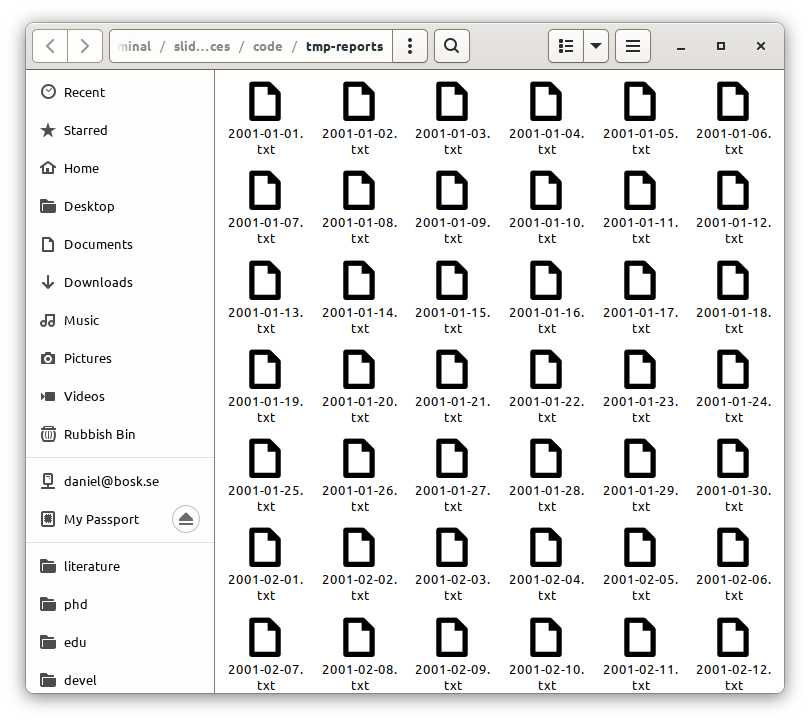
\includegraphics[height=0.5\textheight]{fig/many-reports.png}
    \caption{file explorer showing many dated report files.}
  \end{figure}

  \begin{exercise}[Printing contents of specific files]
    \begin{itemize}
      \item Take the contents of all reports from summers of 2005--2008.
      \item Put into one file.
    \end{itemize}
  \end{exercise}
\end{frame}

\begin{frame}[fragile]
  \begin{figure}
    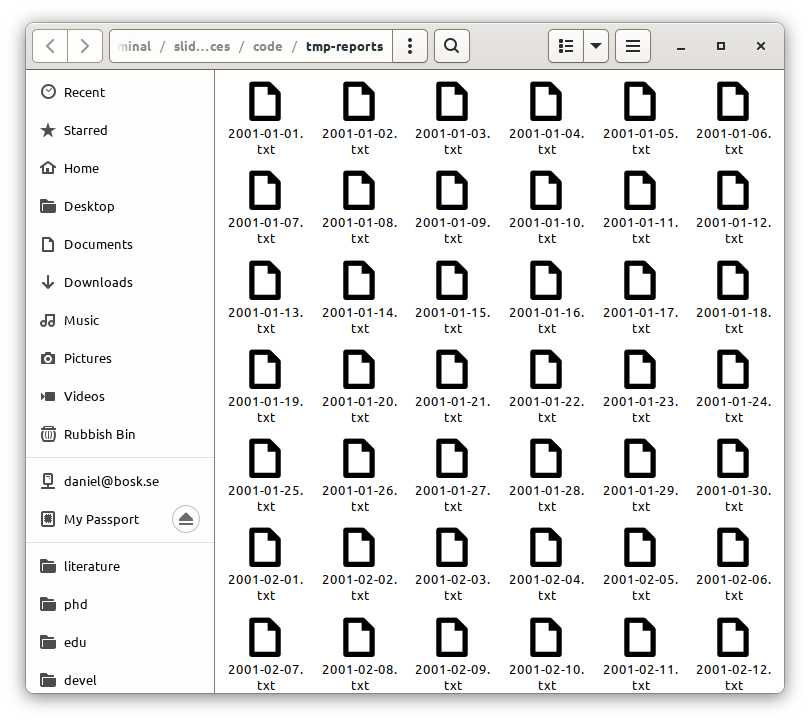
\includegraphics[height=0.5\textheight]{fig/many-reports.png}
    \caption{file explorer showing many dated report files.}
  \end{figure}

  \begin{solution}[CLI-solution: \texttt{summer.sh}]
    \inputminted[firstline=3]{bash}{code/summer.sh}
  \end{solution}
\end{frame}


\section{Scripting}

\begin{frame}
  \begin{figure}
    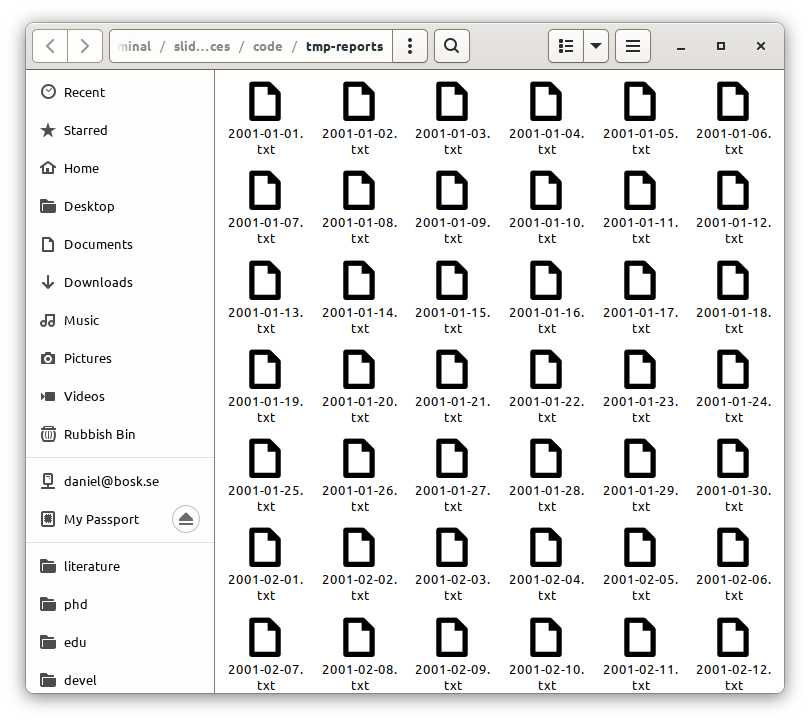
\includegraphics[height=0.5\textheight]{fig/many-reports.png}
    \caption{file explorer showing many dated report files.}
  \end{figure}

  \begin{exercise}
    \begin{enumerate}
      \item Sort the reports into subdirectories, one directory per year.
      \item For each year, sort the reports into the subdirectories: summer, 
        autumn, winter and spring.
    \end{enumerate}
  \end{exercise}
\end{frame}

\begin{frame}[fragile]
  \begin{example}[Positional arguments, \texttt{args.sh}]
    \begin{itemize}
      \item \texttt{args.sh:}
    \end{itemize}
    \inputminted[linenos,highlightlines={2,3}]{bash}{code/args.sh}
    \begin{itemize}
      \item \texttt{bash args.sh one two three}
    \end{itemize}
    \begin{minted}[highlightlines={2,3}]{text}
fixed: one two three
order: one two three
unorder: three two one
    \end{minted}
  \end{example}
\end{frame}

\begin{frame}[fragile]
  \begin{example}[\texttt{vars.sh:}]
    \inputminted[linenos,firstline=3,highlightlines={5,6}]{bash}{code/vars.sh}
  \end{example}
\end{frame}

\begin{frame}[fragile]
  \begin{solution}[Sorting the reports]
    \inputminted[linenos,firstline=3,lastline=11,highlightlines=3]{bash}{code/sort.sh}
  \end{solution}
\end{frame}

\begin{frame}
  \begin{remark}
    \begin{itemize}
      \item The grading scripts are written like this.
    \end{itemize}
  \end{remark}

  \begin{example}[Grading terminal assignment]
    \inputminted[linenos,firstline=55,lastline=70,fontsize=\scriptsize]{bash}{code/grade.sh}
  \end{example}
\end{frame}

\printbibliography
\end{document}
